\chapter{DESIGN/DATA COLLECTION}\label{chap3}
\thispagestyle{empty}

The survey conducted in Government Engineering College Bartonhill was done using the open source tool Open Data Kit (ODK). This chapter explores Open data Kit, workflow of ODK for ppvm.  
\section{ODK: A brief Introduction}

%A figure can be inserted as follows. Fig.~\ref{figureone} is in this section and so on...... First observe the figure number should contain the chapter number as the first digit and the second digit or number as the position of the figure in the current chapter.  
The Open Data Kit (ODK) community produces free and open-source software for collecting, managing, and using data in resource-constrained environments. It allows for the collection of data offline and submission of the data when internet connectivity is available. It allows communities to aggregate data with full control over the collected data and the servers where this data is stored. \cite{odk}


\begin{figure}[h!]
\centering
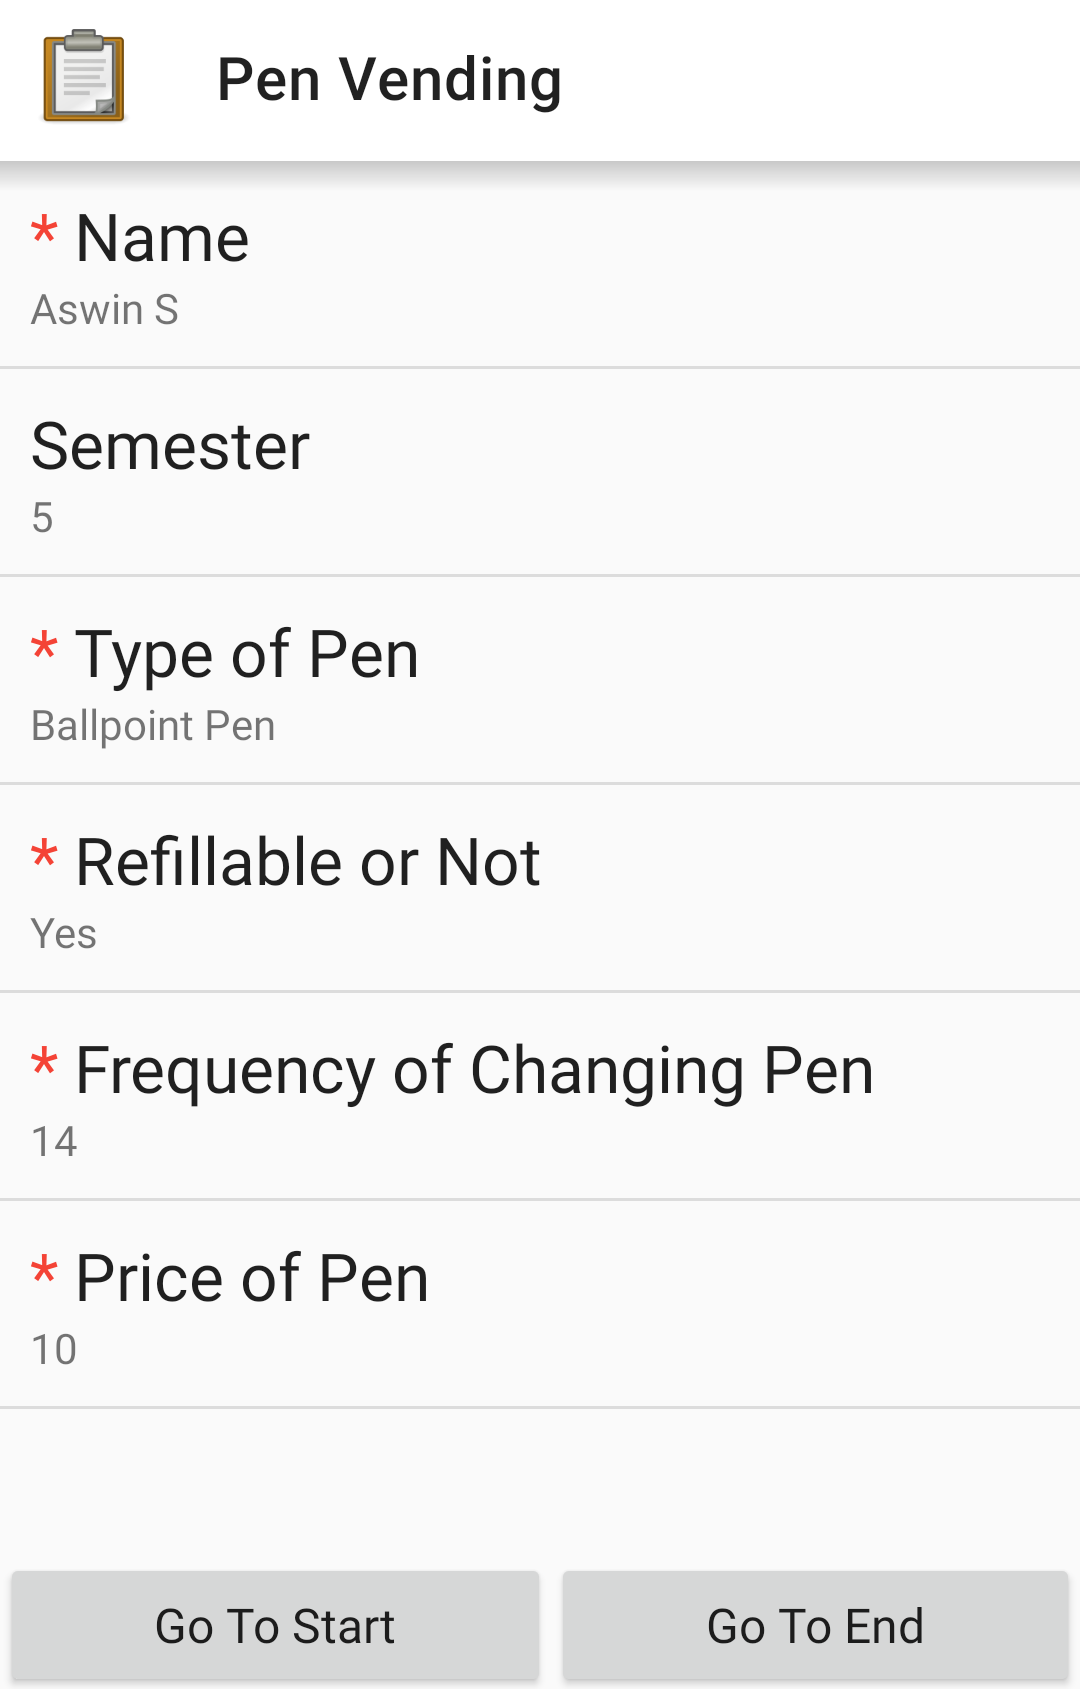
\includegraphics[width=0.4\linewidth]{./picture-files/odk.png}
\caption[ODK-Collect]{Interface of ODK-Collect}
\label{figureone}
\end{figure}

%See how the figure in this chapter is used in another chapter to refer to it by its number and page number. Check Chapter~\ref{chap4}, page no.~\pageref{chap4}.

\section{Components of ODK}
   \begin{itemize}
  \item \textbf{ODK-Collect}: Android Open Source App for Data Collection even for offline use in remote areas without internet connectivity.
   \item \textbf{ODK Build}: Component is used for designing a questionnaire for ODK. It works as a drag-and-drop form designer for ODK XForms. It is used for data collection campaign e.g. for Health Sites
 \item \textbf{ODK Aggregate}: The ODK Aggregate is the backend of ODK infrastructure, receiving the data from the mobile devices. To be multiplatform it is designed as Open Source Java server, that stores, analyzes, and presents survey data. Decision support is build on the collected data.   
\end{itemize}   

\section{Workflow for data collection}
   \begin{itemize}
  \item Download or Create a questionnaire for data collection, which is available for offline use.
   \item Collect the data, even if device is offline.
    \item Submit collected data to ODK Aggregate.
    \item Access aggregated results for individual decision support (optional).
\end{itemize} 


%Here in this section you can give a proper name and explain about it. 

%We can see a sample table, Table~\ref{tableone}, in page no.~\pageref{tableone} referred in this section. Any floating objects like this can be referred without actually counting the page where it comes in the document. Just say what to be done, the rest is up to \LaTeX. % will do the rest.
%\begin{table}[h!]\centering \caption{Expenses of Rakhul}\label{tab-exp}
%\begin{tabular}{|l|r|r|r|}
%\hline 
%Item	&	Rate	&	Qty.	&	Amount	\\ \hline
%Rice	&	34	&	5	&	170	\\ \hline
%Sugar	&	32	&	1	&	32	\\ \hline
%Salt	&	15	&	1	&	15	\\ \hline
%Chilli	&	150	&	0.25	&	37.5	\\ \hline
%	&		&	Total	&	254.5	\\ 
%	\hline
%\end{tabular}

%\end{table}

%\begin{table}[h!]\centering \caption{Modifications in a table design}
%\begin{tabular}{||c||c||c||c||c||}
%\hline Rakhul & Vrinda & Raveendran & Krishna & Anu \\ 
%\hline  &  &  &  &  \\ 
%\hline  &  &  &  &  \\ 
%\hline  &  & Anna & Bhaskar & Nizam \\ 
%\hline 
%\end{tabular} 
%\end{table}


%In Section~\ref{e-proc}, page no.~\pageref{e-proc}, the different modes and different practices in e-procurement has been discussed. The research in e-procurement actually discusses the success stories of e-procurement.
\subsection{Workflow for data collection of PPVM}
\begin{itemize}
\item A form was created using odk build and was saved to ODK server. \item This form was exported as a .xml(eXtensible Markup Language) format file was used with ODK collect android app to carry out the survey.
\item The data collected was saved within the ODK-collect app and the save was finalised at the end of the survey. 
\item This finalised data was then uploaded to ODK aggregate sand box server. 
\item The data uploaded was  exported as .csv(comma seperated values) format file and opened using spreadsheet to do further estimations.

\end{itemize}


\subsection{Survey}

The survey conducted within Government Engineering College Barton Hill was carried out with ODK collect android application. The data collected consists of the following fields:
\begin{itemize}
\item Type of pen.
\item Whether refillable or not.
\item Frequency of changing of pen.
\item Price of pen.
\end{itemize}
The data collected is given in Appendix \ref{ap2}

\section{Data Analysis}

%Any equation in the report can be referred anywhere like this. Eqn.~\eqref{dist}, page no.~\pageref{dist}  is a sample equation that says about the displacement of an object travelling with specific parameters. 
From the data collected the following estimations were deduced per person:
\\Average frequency of throwing a pen, $f$ = 16 days\\
$\therefore$ Number of pens thrown in a day = $\frac{1}{f}$= $\frac{1}{16}$ \\
$\implies$ Number of pens thrown in a year $n_t$ = $\frac{1}{16}\times 365\approx 23$ \\
Now,\\
Approximate population of campus $P$= 1400\\
Total pens thrown per year in college, $N_t$ = $n_t \times P$ = 23 $\times $ 1400 = 32,200 \\
Average weight of plastic pen $w_1$= 6 gm = 0.006kg\\
Thus, weight of all pens thrown in a year $W_1$ = $n_t \times w_1$ =   32,200 $\times$ 0.006 kg = 193 kg\\
Amount of CO$_2$ by burning 1 kg of plastic pens $c_1$ = 6 kg\\
Estimated amount of CO$_2$ emitted per year within the campus $C_1$ = $c_1 \times W_1$ = 1,159 kg\\
Ratio of plastic pens accepted to the paper pens given = 3:1\\
Number of paper pens placed in the machine $N_p$= $\frac{N_t}{3}$ = 10,733\\
Weight of a paper pen $\approx$ Weight of a plastic pen $w_p$ = 0.006 kg\\
Total weight of paper pens given $W_p$= $N_p \times w_p$ = 64.4kg\\
Amount of CO$_2$ by burning 1 kg of paper pens , $c_2$ = 0.6 kg\\
Estimated amount of CO$_2$ emitted by paper pens per year within the campus,\\ $C_2$ = $c_2 \times W_p$  = 38.6 kg\\
Estimated difference in emission of CO$_2$, $C_1-C_2$ = 1120.4 kg

\section{PPVM Design}
For the prototype, it was decided that a combination of both acrylic sheet and foam board would be the best, Fig \ref{fig:ppvm_body}. The front of the machine had to be white, so as to provide a white background while taking the image. The sides of the machine was made with transparent acrylic sheet. A transparent box with tiltable base was attached to the interior of the machine. It was open from the top so that the pen can be entered. The ramp on which the paper pens are stored and rolled out are made with foam board. The rotating part is done using servo motors. The camera and the Raspberry Pi are attached inside.

\begin{figure}[H]
	\centering
	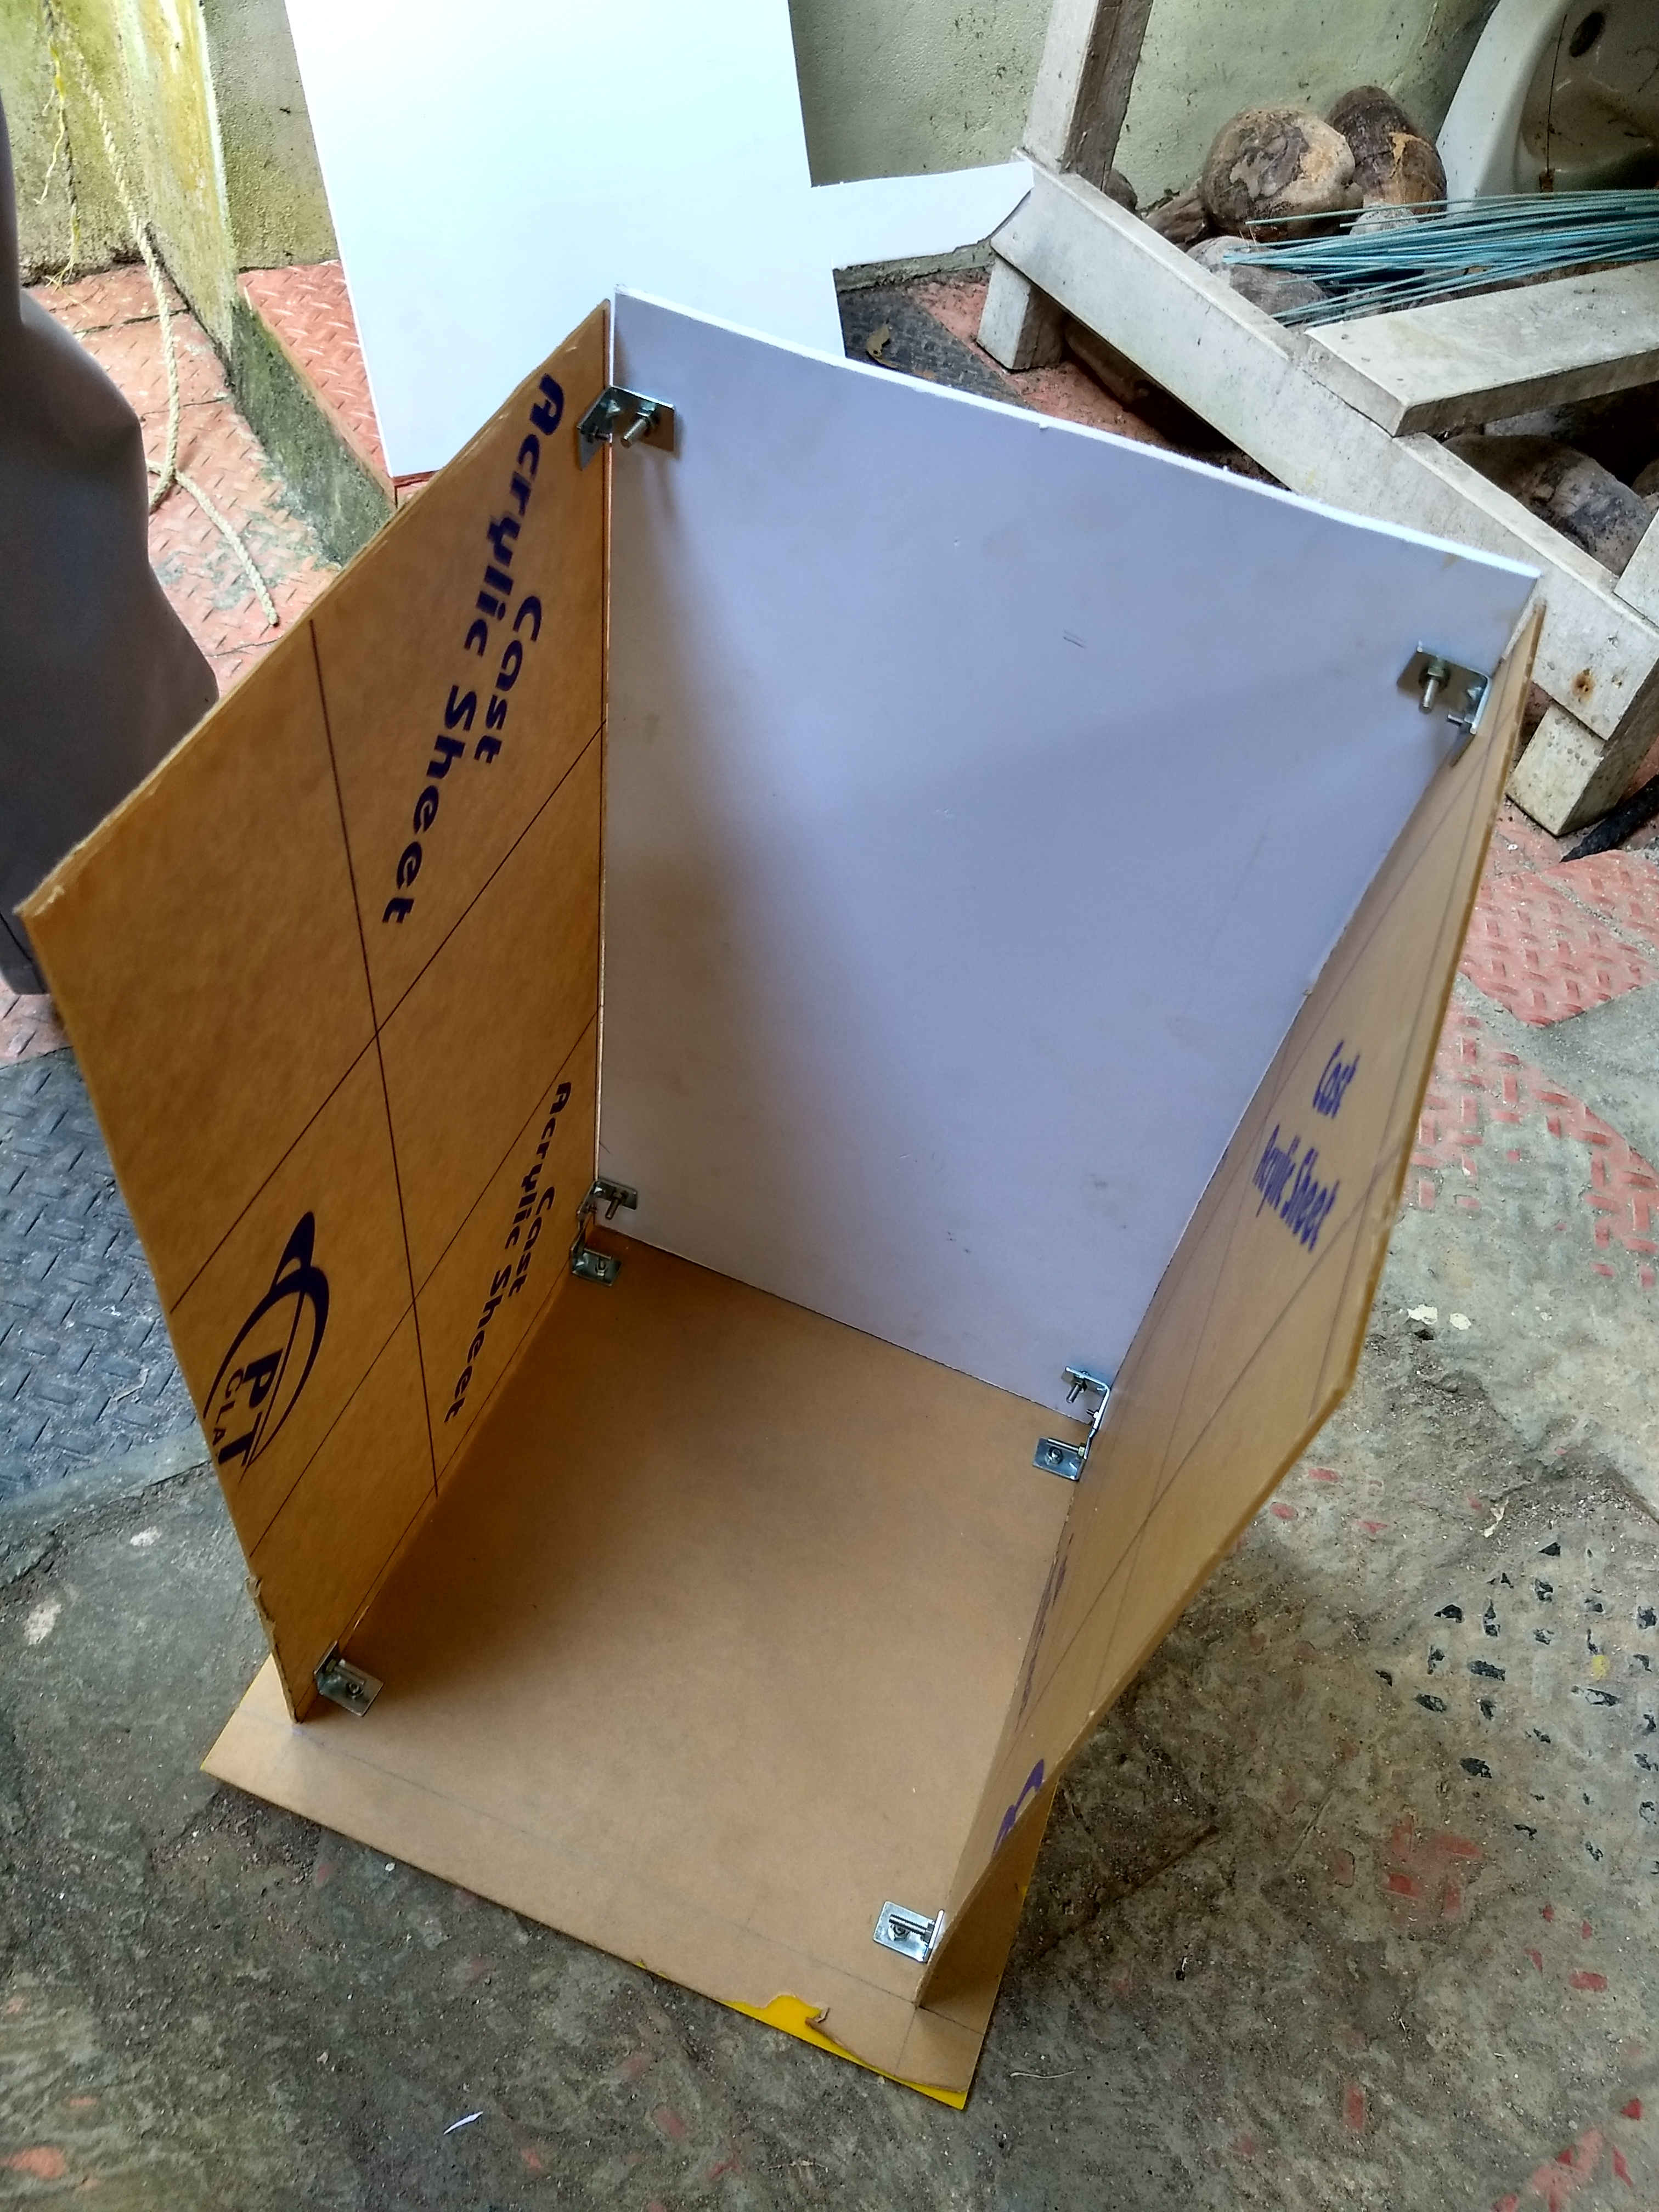
\includegraphics[width=0.7\linewidth]{./picture-files/ppvm_body.jpg}
	\caption{PPVM body}
	\label{fig:ppvm_body}
\end{figure}


\section{Estimation}

\begin{table}[H] \caption{Table showing the cost estimation}
	\centering
	\begin{tabular}{|c|c|c|c|}
		\hline 
		\textbf{ Sl. No.}&\textbf{Component}&\textbf{Quantity}	&\textbf{Price}\\ \hline
		1& Acrylic Sheet (2mm)	&	6 sq. ft.	&	550	\\ \hline
		2& Foam Board (5mm)	&	4 sq. ft.	&	160		\\ \hline
		3&Raspberry Pi 4 (1 GB)	&1	&3400		\\ \hline
		4&Raspberry Pi camera	&	1	&	1900		\\ \hline
		5&Servo Motors (MG995) 	&	1	&	700	\\ \hline

			&	\textbf{Total}	&		&	6710	\\ 
		\hline
	\end{tabular}
	
\end{table}


\begin{comment}

\begin{figure}[H]
	\centering
	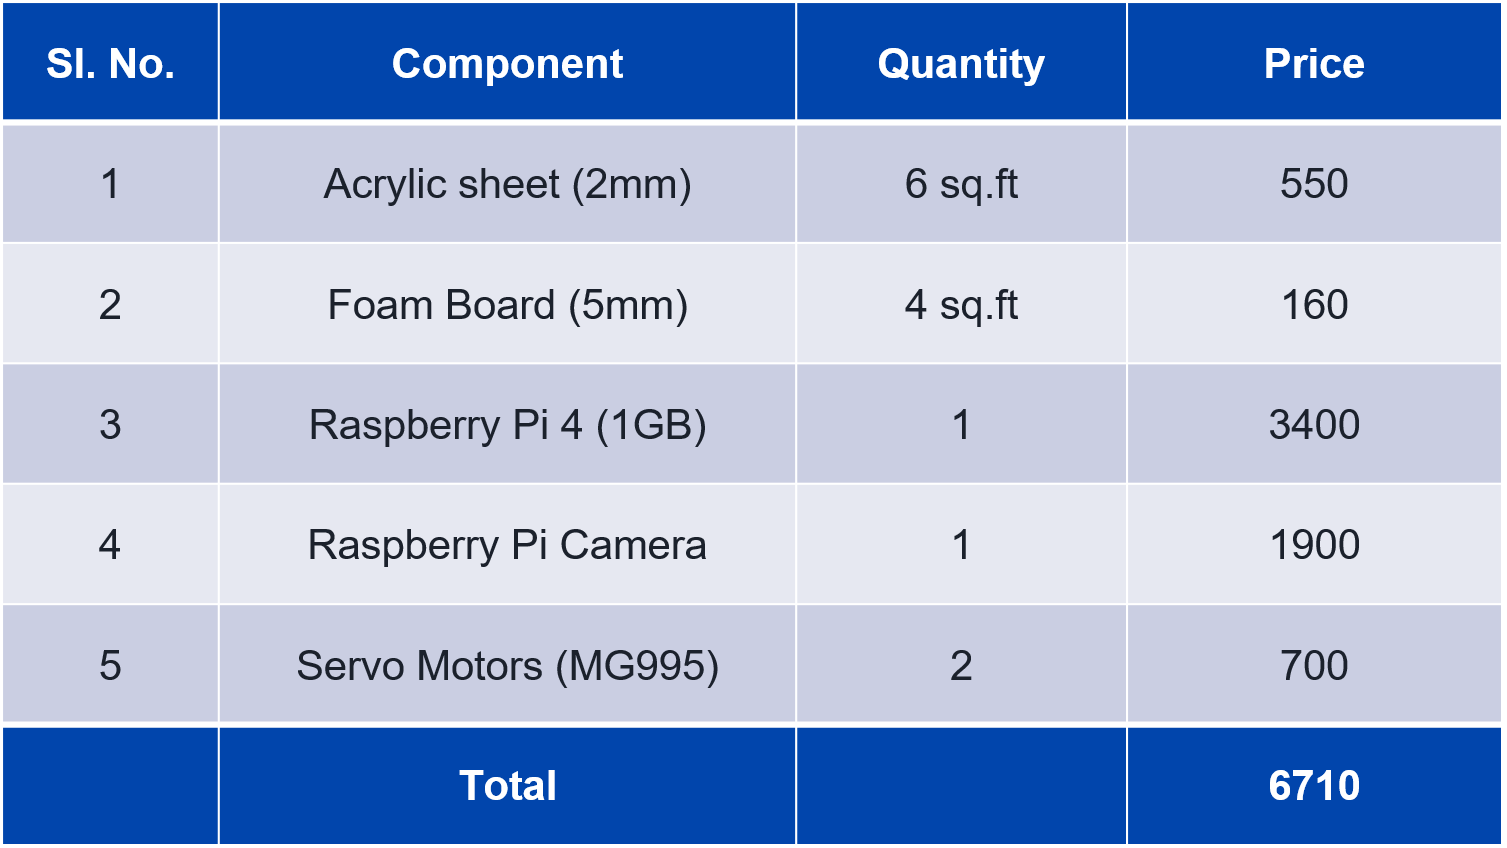
\includegraphics[width=0.85\linewidth]{./picture-files/estimation.png}
	\caption{Cost estimations}
	\label{fig:estimation}
\end{figure}
\end{comment}
\section{Summary}


%Provide a paragraph to summarise every chapter.
\begin{itemize}
\item Data was collected using ODK-Collect.
\item The collected data was used to estimate the amount of CO$_2$ prevented from releasing to atmosphere.
\item Estimated manufacturing cost: Rs. 6,710.
\item Prototype made with a combination of acrylic sheet and foam board.




\end{itemize}


% 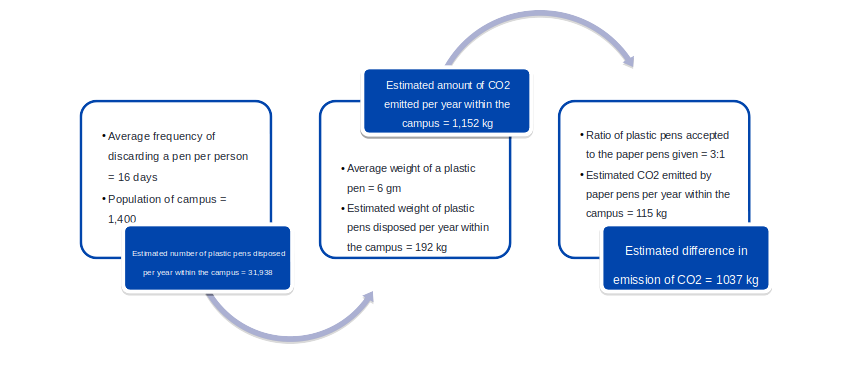
\includegraphics[width=1.3\linewidth]{./picture-files/pptpic.png}

